\section{Requisitos}
Como la metodología de desarrollo ha sido iterativa, algunos de los requisitos han ido surgiendo durante el desarrollo de la aplicación, e inclusos algunos requisitos han cambiado según se han ido encontrando o destruyendo barreras. Los requisitos iniciales, que se plantearon en la primera reunión eran:

Desarrollar una aplicación para cuatro jugadores en las que compiten para encontrar la palabra. En este momento ya se ha definido que es un juego variante del Wordle, además, por simplificar el desarrollo en estos momentos iniciales, se ha decidido guardar la información sobre los jugadores en memoría, sin utilizar ninguna base de datos.

\subsection{Fases}
En cada fase de desarrollo quedan agrupadas una serie de nuevos requisitos y mejoras sobre los requisitos que ya se habían completado.

\subsubsection{Fase 0}
En la fase 0, se propone la idea de la aplicación y se comienzan a crear requisitos, primero se define las ideas y los requerimientos, como la necesidad de crear un sistema de tiempo real, además, se especifican las tecnologías, y se define como debería de avanzar el proyecto a lo largo del tiempo.

\subsubsection{Fase 1}
En la fase 1, se presentó una primera versión de la aplicación, en ella un número no controlado de jugadores podían jugar en una misma sala, existía un lobby donde los jugadores podían cambiar su nombre y podían jugar hasta que uno ganase. Todavía no se llegaba a controlar el que los jugadores hubieran perdido, así que era posible quedarse bloqueado con todos los jugadores sin posibilidad de probar nuevas palabras.
La palabra objetivo en esta fase no era generada aleatoriamente, en su lugar, era siempre la misma palabra. Esto facilitaba mucho las pruebas iniciales de flujo de la aplicación.

\subsubsection{Fase 2}
En la fase 2, el servidor ya era capaz de generar una palabra aleatoria entre una lista de posibles palabras. Todos los jugadores reciben la palabra objetivo aleatoria al comenzar la partida, en el momento en el que uno de ellos ganaba, se mostraba su nombre y la palabra objetivo en una nueva página.
	      	      	      	      	      	      	      	      
La página que muestra al jugador ganador, como el resto de páginas, fue cambiando a lo largo del tiempo, sobre ella se hicieron muchas iteraciones que permitieron llegar al diseño final.

\subsubsection{Fase 3}
En la fase 3, se introdujo la opción de unir a traves del boton de Join del menú principal, además, se introdujo la posibilidad de ver en tiempo real el conocimiento adquirido de cada jugador sobre la palabra objetivo y se amplió la lista de palabras para que soportara diferentes idiomas, en concreto se introdujo el idioma español, pero el sistema es capaz de introducir nuevas listas de palabras de manera sencilla.
	      	      	      	      
Además, se prestó especial atención a casos donde hay un único jugador en la partida, por ejemplo, para estos casos se eliminó la cuenta atrás del principio de la partida.
	      	      	      	      	
Para poder probar con amigos y compañeros de trabajo, se desplegó la aplicación moviendo las aplicaciones a un servidor de DigitalOcean, levantando ambas aplicaciones utilizando los comandos que proveen tanto SvelteKit como Deno. Esta forma de levantar las aplicaciones se demostró muy lenta, ya que requería actualizar los repositorios del servidor usando Git, para después compilar y ejecutar las aplicaciones.

\subsubsection{Fase 4} Para la fase 4, se arreglaron bugs presentes, además se desarrolló la posibilidad de levantar la aplicación utilizando Docker y Docker Compose.

En este momento la aplicación ya se encontraba con madurez suficiente para que los cambios necesarios fueran aplicados sin necesidad de hacer refactorizaciones ni grandes cambios en los sistemas de la aplicación.    	      	      	      	      	


\section{Arquitectura general}
El proyecto está dividido en dos repositorios, por un lado está la aplicación web (webapp), que se encarga de realizar la lógica de presentación, así como el game loop, y por otro lado tenemos el servidor de backend, donde va toda la lógica de websockets en la parte de servidor.

La comunicación entre aplicaciones se realiza mediante peticiones HTTP y websockets, para ello se utiliza la librería estándar de Javascript proporcionada por el navegador, la librería estándar de Node.js, la librería estándar de Deno y la librería Socket.io.


\begin{center}
	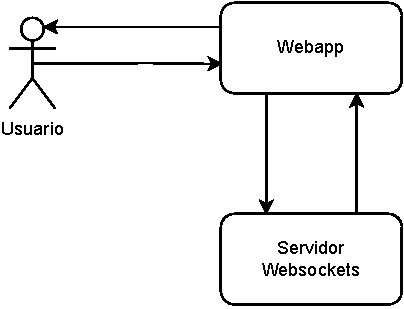
\includegraphics[clip=true,width=0.5\textwidth]{./diagrams/general_arch.pdf}
\end{center}

\subsection{Aplicación web}
La aplicación web es la herramienta con la cual el usuario interactúa, permite a este realizar todas las acciones necesarias utilizando un navegador web.

Está desarrollada utilizando SvelteKit para la realización de la lógica, y Tailwind para dar color y estilo.

El flujo principal que sigue el usuario para poder jugar una partida comienza abriendo la página web de la aplicación web, después, creará o se unirá a una partida ya creada, cuando todos los jugadores estén listos, el creador de la partida le dará al botón de comenzar, y después de una cuenta atrás, a todos los jugadores se les presentará un tablero de Wordle donde pondrán ir escribiendo sus intentos. Si alguno de los jugadores descubre la palabra, todos los jugadores verán una nueva pantalla con el nombre de la persona ganadora, en esta nueva pantalla, los jugadores pueden elegir entre salir de la partida o volver a jugar. En caso de que ningún jugador consiga ganar, se les presentará a todos una pantalla en el que se mostrará la palabra objetivo, y las mismas opciones que en el caso de haber habido un ganador.


\begin{center}
	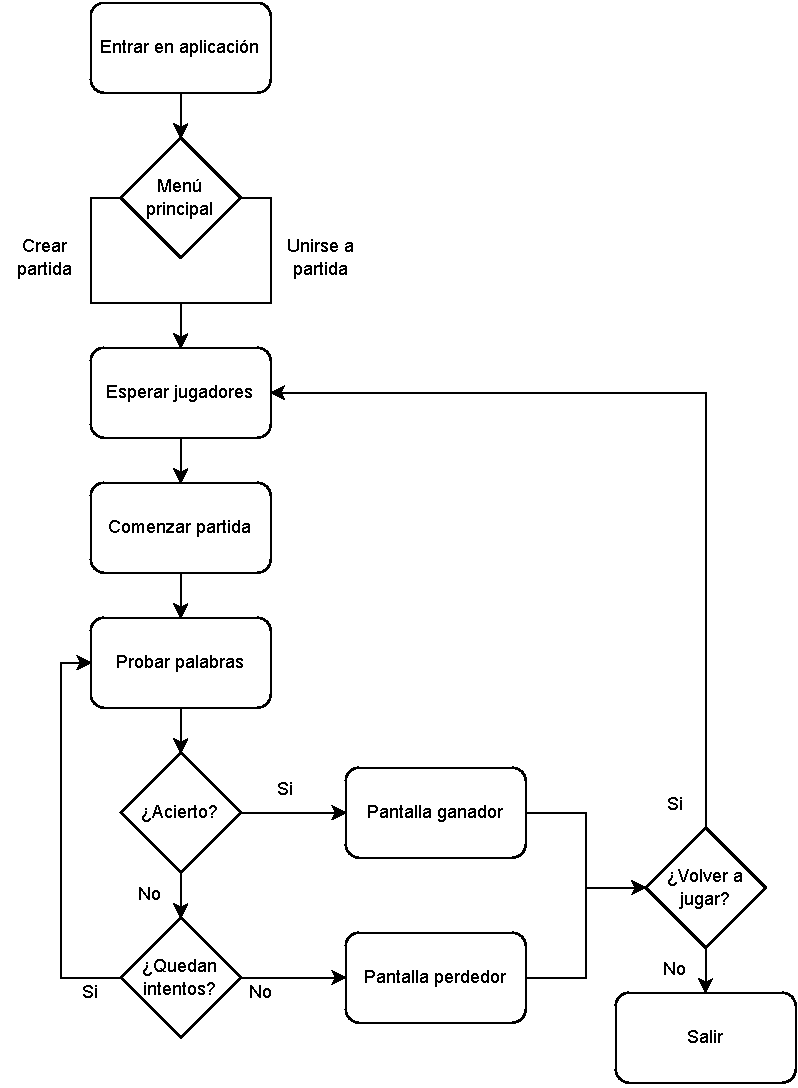
\includegraphics[clip=true,width=\textwidth]{./diagrams/webapp_flow.pdf}
\end{center}

\subsubsection{Comunicación websocket}
La comunicación websocket ha sido el punto de aprendizaje principal, según se fueron desarrollando las diferentes partes para el trabajo, se fue definiendo lo que acabó siendo una serie de reglas sobre la comunicación diferenciando estas en tres tipos de comunicación diferentes.

Para entender estos tres tipos de comunicación hay que entender primero el sistema de comunicación HTTP. En este tipo de comunicación es el cliente el que inicia la llamada y es el servidor el que responde a esta. Sin embargo, en websockets, el servidor puede enviar información al cliente sin que sea el iniciador de la llamada. Por ello Websockets funciona por sistemas de eventos, donde el socket puede enviar y esperar comunicación (comunicación bidireccional).

Una vez entendida la comunicación HTTP y la comunicación websocket, y las diferencias entre ambas, va a quedar claro porque en CoWordle se diferencia entre tres tipos distintos de comunicación.

En primer lugar tenemos la comunicación cliente - servidor, donde el cliente envía eventos al servidor, y el servidor puede actuar ante estos eventos, pero no responde a través de ellos. 
Estos eventos se clasifican como eventos OUT, ya que el cliente envía información al exterior. Por ejemplo, la llamada cuando un jugador ha sido expulsado de la partida (\textit{remove\_player}), se envía desde el host de la partida hacia el servidor, cuando el servidor ha procesado este evento, envía a todos los jugadores de la partida el evento \textit{player\_disconnected}, y serán los clientes los que eliminen de sus listados locales al jugador que se ha eliminado.

En segundo lugar tenemos la comunicación servidor - cliente, un ejemplo de esto es el recién descrito \textit{player\_disconnected}, en el que el servidor envía un evento a los jugadores de la sala. Este tipo de eventos se clasifica en CoWordle como IN, porque el cliente recibe información del servidor.

Por último lugar el último tipo de comunicación se clasifica como DIALOGUE, y se explica porque es comunicación cliente - servidor - cliente, es decir, es el cliente el que comienza la comunicación, el servidor procesa la respuesta y se la envía al cliente con el mismo nombre de evento con el que la llamada había comenzado, hasta que la llamada no ha sido respondida, el cliente se quedará esperando una respuesta de manera asíncrona, es decir, sin bloquear al resto de la aplicación.

\subsection{Servidor Websockets}
El servidor de websockets está implementado utilizando Deno y una librería que ayuda al manejo de eventos para los websockets llamada Socket.io. Deno se utiliza para levantar el servidor y para recibir peticiones HTTP, aunque existen pocos endpoints para la comunicación HTTP, existe un endpoint necesario para que Socket.io cree la conexión de Websockets, y uno más para la creación de la partida.

\subsubsection{Sistema de eventos}
El servidor responde a peticiones HTTP y de Websockets creando eventos que son respondidos de manera secuencial por funciones lambda, cada función sólo responde a un evento, devolviendo una respuesta.
Javascript es una tecnología uni-hilo, pero es capaz de realizar concurrencia utilizando primitivas asíncronas llamadas promesas, cuando una función marcada como asíncrona se ejecuta, el motor de Javascript la guarda como evento, este evento será manejado cuando el motor de Javascript lo considere oportuno. Por ejemplo, cuando la CPU está esperando una lectura de la memoría, Javascript puede cambiar el contexto y procesar otras funciones. De está manera, Javascript es capaz de maximizar la utilización de su hilo de ejecución.

\subsubsection{Eventos disponibles}
El servidor permite la comunicación utilizando las siguientes rutas HTTP:Soso

\begin{itemize}
	\item \textit{/create-route}, genera un nuevo identificador de partida. Este identificador es fundamental para la comunicación entre el cliente y el servidor ya que permite la identificación de la partida para realizar las operaciones necesarias.
	\item \textit{/testing/solution}, este endpoint está disponible para poder realizar un tests de integración de flujo completo.correcta.
\end{itemize}

A parte de las rutas HTTP, el servidor permite la comunicación Websocket utilizando los siguientes eventos:

\begin{itemize}
	\item \textit{setup} es un evento de tipo diálogo que une a un jugador a la partida, es necesario enviar como parámetros el código de la sala generado por /create-room y el nombre del usuario que se va a unir a la partida, este evento avisa a todos los demás jugadores de la sala que se ha unido el jugador emitiendo el evento \textit{player\_connection}.
	\item \textit{update\_player\_name} es un evento de tipo diálogo que permite a los jugadores actualizar su nombre, especialmente útil porque el primer nombre que recibe cada jugador al conectarse a la partida es aleatorio entre una combinación de posibilidades.
	\item \textit{remove\_player} es un evento de tipo out que solo pueden utilizar el creador de la partida, y permite expulsar a jugadores de la partida. Cuando ha expulsado a un jugador emite un evento \textit{player\_disconnected} que notifica al resto de usuarios de la desconexión.
	\item \textit{validate\_word} es un evento de tipo diálogo que comprueba un intento de un jugador con la palabra objetivo. El resultado de la operación de comprobación es un array de una enumeración (\textit{WordlePoints}) que indican el resultado de cada letra en la palabra (si no se encuentra en la palabra, si se encuentra en la palabra, si está en la posición correcta). Este resultado se envía directamente al jugador que ha ejecutado el evento, pero también se envía a los demás jugadores para indicar en el scoreboard el conocimiento de cada jugador. Además, se comprueba si la partida ha terminado por que el intento coincide con la palabra objetivo, y si todos los jugadores han perdido porque se han quedado sin intentos.
	\item \textit{start\_game} es un evento de tipo out que permite al host de la partida empezar. En el momento que se lanza este evento todos los jugadores reciben el evento \textit{start\_prematch} que les indica cuándo comenzará la partida.
	\item \textit{disconnect} es un evento nativo de Socket.io, que permite al servidor conocer cuando un jugador se ha desconectado de la partida, existen varias razones para que se ejecute este evento, por ejemplo, que el jugador haya perdido la conexión con internet, o que el jugador haya decidido abandonar la partida cerrando el navegador. En este evento se comunica al resto de jugadores que este ha abandonado la partida, en caso de ser el jugador que ha creado la partida el que la abandona, se cierra también para el resto de jugadores.
\end{itemize}


\subsubsection{Endpoints HTTP}
Como el objetivo del trabajo era el aprendizaje de la comunicación bidireccional, la mayor parte de la comunicación se realiza a traves de websockets, aun asi existen dos rutas disponibles para la realización de comunicación HTTP:

\begin{itemize}
	\item \textit{/create-room} crea una nueva partida para que los jugadores puedan unirse y jugar. Cada partida está identificada por un identificador que se genera durante este proceso.
	\item Existe también una ruta reservada por la librería de Socket.IO que se utiliza internamente para establecer la conexión websocket. Esta ruta está completamente manejada por Socket.IO.
\end{itemize}

\subsubsection{Identificador de partida}
Cada partida tiene un identificador único de seis cifras generado pseudo-aleatoriamente llamado roomCode. El roomCode lo generará el servidor de websockets tras la petición de /create-room, este endpoint HTTP únicamente reserva el código generado para la partida, utilizando ese código los jugadores son capaces de unirse a la partida inicialmente, el código también se utiliza para realizar la comunicación cliente-servidor.


\section{Diseño e Implementación}

\subsection{La reutilización de componentes}
Svelte, la tecnología que he usado para hacer los componentes de front, se basa en la creación de componentes que puedan ser reutilizados en diferentes situaciones, la reutilización de código se considera buena práctica en todo el ámbito de la ingeniería informática. Por ello parece importante destacar que una buena elección de la tecnologías es solo la base, y es necesario hacer un buen uso de estas para poder llegar a un buen resultado, por ello en este apartado quiero destacar un buen uso de componentes de Svelte.

Existe un componente que se reutiliza varias veces a lo largo de la aplicación, el componente llamado <Word>, que se encuentra en el archivo Word.svelte de la aplicación cowordle-webapp.

Este componente se utiliza como botones estilizados en el menú principal, en este primer uso, el componente muestra la palabra elegida por el desarrollador, indicando al usuario que es un botón con el que puede interaccionar.

\begin{figure}[H]
	\centering
	
\includegraphics[clip=true]{images/reusing/host_component.png}
	\caption{Imagen del componente como botón.}
	\label{fig:comp_host_image}
\end{figure}

Después, se vuelve utilizar como huecos para las palabras mientras se juega, en este caso la palabra tiene distinto número de huecos disponibles, además está completamente vacía de texto.

\begin{figure}[H]
	\centering
	
\includegraphics[clip=true, width=0.75\textwidth]{images/reusing/empty_component.png}
	\caption{Imagen del componente con texto vacio.}
	\label{fig:comp_empty}
\end{figure}


Cuando el jugador interacciona con el teclado mientras juega, las palabras se van llenando de letras.

\begin{figure}[H]
	\centering
	
\includegraphics[clip=true, width=0.75\textwidth]{images/reusing/filled_component.png}
	\caption{Imagen del componente con texto.}
	\label{fig:comp_filled}
\end{figure}

Además, las letras muestran el progreso de la palabra objetivo, utilizando los colores característicos.

\begin{figure}[H]
	\centering
	
\includegraphics[clip=true, width=0.75\textwidth]{images/reusing/colored_component.png}
	\caption{Imagen del componente con texto y colores.}
	\label{fig:comp_colored}
\end{figure}

Todas las imágenes mostradas representan el mismo componente de Svelte, y permiten mostrar las ventajas de utilizar tecnologías web reactivas.
Comenzando por el principio, necesitamos un componente que sea capaz de mostrar texto.

\begin{figure}[H]
	\centering
	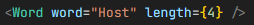
\includegraphics[clip=true, width=0.6\textwidth]{images/reusing/code_simple_component.png}
	\caption{Imagen código para utilizar el componente.}
	\label{fig:comp_simple_code}
\end{figure}

Así es como se utiliza el componente Word, para mostrar el texto de la primera imagen simplemente es necesario definir la palabra a mostrar y su longitud.

También queremos que el componente reciba texto del usuario dinámicamente, esto sería posible reprogramando al componente o creando uno nuevo, pero realmente ya tenemos esta funcionalidad sin necesidad de programar nada más. En lugar de utilizar como argumento para el parámetro word un string fijo, podemos utilizar una variable, e indicarle a Svelte que esa variable es reactiva utilizando, la directiva bind, que recalcula el componente cada vez que cambia el contenido de la variable pasada.

\begin{figure}[H]
	\centering
	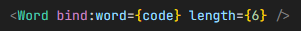
\includegraphics[clip=true, width=0.75\textwidth]{images/reusing/code_dyn_component.png}
	\caption{Imagen código para utilizar el componente con texto dinámico.}
	\label{fig:comp_dyn_code}
\end{figure}

En este caso estamos utilizando la directiva bind para hacer que el componente se redibuje cada vez que cambia la variable code. Esto significa que nuestro componente es ajeno al texto que presentamos, y es responsabilidad de otros componentes seleccionar el texto a mostrar.

Parece un pequeño detalle, pero esta flexibilidad de desarrollo simplifica el código haciéndolo muy reutilizable y componible.

La primera implementación del componente Word se hizo cuando se comenzó el proyecto,  y sin mucho cambio, ha llegado a utilizarse en otras partes de la aplicación en las que no se había llegado a pensar cuando se creó el componente, y eso demuestra que se realizó un buen diseño inicialmente.

\subsection{Tipados en la comunicación websocket}
Como se ha explicado en el apartado XX, la comunicación websocket con el servidor de CoWordle se clasifica en tres grupos, según sea cliente - servidor, servidor - cliente y cliente - servidor - cliente. En este apartado se va a explicar cómo de fácil es realizar esta comunicación independientemente del tipo de esta.

Toda esta capa de tipado se construye como un wrapper sobre el socket expuesto por Socket.IO, esto permite utilizar la potencia de Socket.IO, mientras se provee la seguridad de tipos y la comodidad se autocompleciones del IDE.

\subsubsection{Comunicación IN}
Para la comunicación IN, es el servidor quien envía el evento al cliente, por ello el cliente debe quedarse esperando a que el servidor envíe la petición.

El wrapper expone un método \textit{on}, que permite añadir un callback cuando el evento sea emitido, es decir, cuando el servidor lo emite y el cliente lo haya recibido.

\begin{mytypescript}[float={!h},caption={Uso de eventos websocket IN.},label={alg:ws_in_usage}]
	this.socket.on("player_connected", ({ newPlayer }) => {
		this.addPlayer(newPlayer);
																														
		this.notifies.playersUpdated.broadcast(this.players);
	}); 
\end{mytypescript}

En el ejemplo del código \ref{alg:ws_in_usage} se puede observar cómo se está definiendo que cuando el evento \textit{player\_connected} ocurra, la función lambda debe ejecutarse. El evento \textit{player\_connected} está declarado utilizando tipos de la siguiente manera:

\begin{mytypescript}[float={!h},caption={Ejemplo de declaración de la comunicación IN.},label={alg:player_connected_type}]
	export type WebsocketInEvent = {
		...
		player_connected: {
			newPlayer: InitialPlayerInfoDto;
		};
		...
	};
\end{mytypescript}

En esta declaración tan solo necesitamos indicar los parámetros que nos van a llegar del servidor, esta declaración de tipos permite dos mejoras con respecto a los eventos directos de Socket.IO. Por un lado, el IDE ofrece ayuda sobre los nombres de los eventos disponibles sobre los que hacer la espera, además, nos ofrecerá ayuda sobre los parámetros que vamos a recibir según el nombre que indicamos en el primer argumento.

Todo esto es posible gracias al poderoso sistema de genéricos proporcionado por Typescript.

\begin{mytypescript}[float={!h},caption={Declaración del método \textit{on}.},label={alg:on_method}]
	on<TEvent extends EventName<WebsocketInEvent>, TArgs extends WebsocketInEvent[TEvent]>(
	event: TEvent,
	callback: (args: TArgs) => void,
	): void {
		this.socket.on(event as string, callback);
	}
\end{mytypescript}

Como se puede ver en la definición del método \textit{on}, el primer parámetro es el nombre del evento, que está tipado como el genérico \textit{TEvent} que está a su vez definido como un nombre de evento de la lista de eventos IN. El segundo parámetro es el callback a que se llamará cuando el evento se ejecute, este parámetro está tipado como una función que recibe un argumento del tipo \textit{TArgs}, que es de la lista de eventos IN, aquel que coincide con la el genérico \textit{TEvent}. Todo ello ofrece suficiente información al IDE para ser capaz de autocompletar todo lo necesario para que el programador esté seguro de lo que está programando es correcto, y además, mejora la mantenibilidad a largo plazo, porque en caso de cambiar el tipado de algún evento IN de la lista de eventos, el cambio sería reflejado automáticamente en toda la aplicación y en caso de que no coincidieran los nuevos tipos con los antiguos, Typescript indicaría al programador donde ha ocurrido el fallo de tipado.

\subsubsection{Comunicación OUT}
La comunicación OUT es aquella que ocurre en dirección cliente - servidor, el cliente solo pretende comunicar información al servidor, sin esperar nada de respuesta.

\begin{mytypescript}[float={!h},caption={Ejemplo de uso del método \textit{emit}.},label={alg:emit_usage}]
	startGame(wordListId: string): void {
		this.socket.emit("start_game", {
			wordListId,
		});
	}
\end{mytypescript}

En este ejemplo, se puede ver cómo se emite un evento al servidor, para emitir un evento necesitamos el nombre del evento a emitir, y necesitamos también la información que queremos enviar por el socket.

Al igual que la comunicación IN, el sistema dispone de un lugar donde definir todos los eventos OUT, para el ejemplo mostrado en la figura anterior, el evento está definido de la siguiente manera:

\begin{mytypescript}[float={!h},caption={Ejemplo de declaración de la comunicación OUT.},label={alg:start_game_type}]
	export type WebsocketOutEvent = {
		...
		start_game: {
			wordListId: string;
		};
	};
\end{mytypescript}

Esta definición es la versión inversa de la mostrada en los eventos IN, lo que declaramos dentro del evento representan los argumentos que vamos a enviar al servidor, mientras que la comunicación IN se definen los argumentos que íbamos a recibir. A pesar de la diferencia de uso, la forma de declarar ambos es la misma.

% vs-code
\begin{mytypescript}[float={!h},caption={Declaración del método \textit{emit}.},label={alg:emit_method}]
	emit<TEvent extends EventName<WebsocketOutEvent>,TArgs extends WebsocketOutEvent[TEvent]>(
	event: TEvent,
	args: TArgs,
	): void {
		this.socket.emit(event, args);
	}
\end{mytypescript}

Si nos adentramos en la declaración del método \textit{Emit}, que como ya hemos visto es el que se utiliza para la comunicación OUT, volvemos a ver la aparición de un tipo genérico \textit{TEvent}, con la diferencia de que este \textit{TEvent} es un evento de la lista de eventos OUT, la otra diferencia con el método \textit{on}, es que en este utilizamos el argumento \textit{args} como el argumento del método \textit{emit} de Socket.IO, que es el que realizara la petición siguiendo el estándar websocket.

El método \textit{emit} ofrece al programador la misma seguridad y mantenibilidad que el método \textit{on}, además, su similitud de uso, ayuda a que sea más fácil usarlo por programadores de todos los niveles.

\subsubsection{Comunicación Dialogue}
En la comunicación de tipo Dialogue, el cliente envía un evento al servidor, esperando una respuesta de vuelta. Este tipo de comunicación es más compleja de implementar que las otras, pero su uso en CoWordle sigue siendo muy simple.

\begin{mytypescript}[float={!h},caption={Ejemplo de uso del método \textit{dialogue}.},label={alg:etiqueta}]
	const { localPlayer, players, hostPlayer } = await this.socket.dialogue("setup", {
		playerName: this.localPlayer.name,
		roomCode: this.roomCode,
	});
\end{mytypescript}

Como se puede ver en el ejemplo, para usar un evento de tipo Dialogue tan solo tenemos que llamar al método \textit{dialogue} del wrapper. El primer argumento define el evento que vamos a emitir y sobre el que vamos a esperar la respuesta. El segundo argumento describe los datos que vamos a enviar. Como respuesta obtendremos una \textit{promesa} de la respuesta que recibiremos del servidor cuando este responda.

Para declarar un evento del tipo Dialogue, se utiliza una sintaxis muy cómoda, que permite diferenciar en un solo vistazo los tipos que vamos a enviar y los tipos que vamos a recibir.

\begin{mytypescript}[float={!h},caption={Ejemplo de declaración del tipo de evento Dialogue.},label={alg:etiqueta}]
	export type WebSocketDialogueEvent = {
		...
		setup: (args: { roomCode: string; playerName: string }) => {
			players: InitialPlayerInfoDto[];
			hostPlayer: InitialPlayerInfoDto;
			localPlayer: InitialPlayerInfoDto;
			roomState: RoomState;
		};
		...
	};
\end{mytypescript}

El evento se declara como una función donde los argumentos son los datos a enviar a servidor, y cuya respuesta son los tipos que vamos a recibir del servidor. 

Como explicaba anteriormente, la implementación es un poco más compleja que en los tipos de comunicación anteriores.

\begin{mytypescript}[float={!h},caption={Implementación del método \textit{dialogue}.},label={alg:etiqueta}]
	async dialogue<TEvent extends EventName<WebSocketDialogueEvent>, TEventMethod extends WebSocketDialogueEvent[TEvent]>(
	event: TEvent,
	params: Parameters<TEventMethod>[0],
	eventResponse?: string
	): Promise<ReturnType<WebSocketDialogueEvent[TEvent]>> {
		return new Promise((resolve, reject) => {
			this.socket.emit(event, params);
																																																
			this.socket.on<string>(eventResponse || event, (result) => {
				this.socket.off(event);
				resolve(result);
			});
																																																
			setTimeout(() => reject("timeout"), 10000);
		});
	}
\end{mytypescript}

El primer parámetro coincide con los de los otros tipos de comunicación, volviendo a usar el \textit{TEvent}. El segundo argumento extrae los parámetros de la función declarada como evento. El valor de retorno del método se define como una \textit{promesa} del valor de retorno definido en función del evento.

Con esta implementación estamos manteniendo la sencillez de uso que teníamos con los otros tipos de comunicación, pero estamos creando una comunicación más clásica, donde el cliente y el servidor se comunican como si fuera una petición HTTP normal.
